
%%%%%%%%%%%%%%%%%%%%%%% file typeinst.tex %%%%%%%%%%%%%%%%%%%%%%%%%
%
% This is the LaTeX source for the instructions to authors using
% the LaTeX document class 'llncs.cls' for contributions to
% the Lecture Notes in Computer Sciences series.
% http://www.springer.com/lncs       Springer Heidelberg 2006/05/04
%
% It may be used as a template for your own input - copy it
% to a new file with a new name and use it as the basis
% for your article.
%
% NB: the document class 'llncs' has its own and detailed documentation, see
% ftp://ftp.springer.de/data/pubftp/pub/tex/latex/llncs/latex2e/llncsdoc.pdf
%
%%%%%%%%%%%%%%%%%%%%%%%%%%%%%%%%%%%%%%%%%%%%%%%%%%%%%%%%%%%%%%%%%%%


\documentclass[runningheads,a4paper]{llncs}




\usepackage{amssymb}
\usepackage{cite}
\setcounter{tocdepth}{3}
\usepackage{graphicx}
\usepackage{url}
\usepackage{float}
\usepackage{subfigure}
\usepackage{array}

\urldef{\mailsa}\path|{hossam.faris}@ju.edu.jo| 
\urldef{\mailsc}\path|erika.siebert-cole,}@ju.edu.jo|    
\newcommand{\keywords}[1]{\par\addvspace\baselineskip
\noindent\keywordname\enspace\ignorespaces#1}

\begin{document}

\mainmatter  % start of an individual contribution

% first the title is needed
\title{SMOTE+Ensembles for Bug Prediction}

% a short form should be given in case it is too long for the running head
\titlerunning{Lecture Notes in Computer Science: Authors' Instructions}

% the name(s) of the author(s) follow(s) next
%
% NB: Chinese authors should write their first names(s) in front of
% their surnames. This ensures that the names appear correctly in
% the running heads and the author index.
%
\author{Hamad, Hossam Faris, Ibrahim and Loai%
\thanks{King Abdullah II School for Information Technology, The University of Jordan, Amman, Jordan}%
\and  \and }
%
%\authorrunning{Lecture Notes in Computer Science: Authors' Instructions}
% (feature abused for this document to repeat the title also on left hand pages)

% the affiliations are given next; don't give your e-mail address
% unless you accept that it will be published
\institute{The University of Jordan\\
Amman, Jordan\\
\mailsa\\
%\mailsc\\
%\url{http://www.springer.com/lncs}}
}
%
% NB: a more complex sample for affiliations and the mapping to the
% corresponding authors can be found in the file "llncs.dem"
% (search for the string "\mainmatter" where a contribution starts).
% "llncs.dem" accompanies the document class "llncs.cls".
%

\toctitle{Lecture Notes in Computer Science}
%\tocauthor{Authors' Instructions}
\maketitle


\begin{abstract}
\keywords{}
\end{abstract}


\section{Introduction}

Today, the task of developing and delivering a bug-free and high quality software product to the end users is becoming more and more challenging. Delivering high quality software product to the end users is ensured by software reliability and software quality assurance \cite{rawat2012software}. With the rapid growth in size and complexity of today's software, the prediction of software reliability plays a crucial rule in software development process \cite{zheng2009predicting}. According to \cite{hall2012systematic,arisholm2010systematic}, the quality of a software product is highly correlated to the presence or absence of the faults. Software fault  presents in a computer program as an error situation that is caused by wrong specification, incorrect programming logic, lack of programming and testing skills, and so forth \cite{dowd2006art,abaei2014survey,tomar2016prediction}. Defective software module hinders the software from working in the desired manner which further increases the development and maintenance costs and is responsible for customer dissatisfaction \cite{fenton2000software,fenton2014software}.

Software defect prediction, which predicts defective software modules, can help the project manager and the software developers in assessing project progress, planning defect detection activities, evaluating product quality and assessing process performance for software management \cite{clark2001good}. Software defect prediction is very useful for finding bugs and prioritizing testing efforts especially when any company does not have sufficient resources for testing the entire product \cite{abaei2014survey,wang2016automatically}. Over the past decades years, a variety of software fault prediction techniques have been proposed \cite{hassan2009predicting,jiang2013personalized,jing2014dictionary, kim2007predicting,lee2011micro,meneely2008predicting,moser2008comparative,nagappan2007using,rahman2013and, wang2012compressed,zimmermann2007predicting,kanmani2007object,khoshgoftaar1999classification,selby1988learning, elish2008predicting,czibula2014software,guo2004robust,agarwal2014prediction,okutan2014software,de2010symbolic, vandecruys2008mining}. In these techniques, researchers have applied several statistical and machine learning techniques to predict the fault proneness models and reduce software development and maintenance costs. Among them, the machine learning technique is the most popular \cite{rawat2012software}. The majority of software fault prediction techniques builds models using metrics and faulty data from an earlier deployment or identical objects and then uses the models to predict whether modules presently under development contain defects, which is called supervised learning approaches \cite{abaei2014survey}.On the other hand, there are other approaches, i.e. clustering, which do not use previous data; these approaches are called unsupervised learning approaches. It is worth pointing out that some researchers, i.e \cite{koksal2011review}; classify software fault prediction techniques into descriptive and predictive techniques.


\section{Related work}

During the last two decades, software defect prediction problem became one of the noteworthy research topic, and increasingly taking great interest from researchers. Many software defect prediction techniques have been developed and applied such as Neural Network \cite{quah2003application}, Support Vector Machine \cite{elish2008predicting}, Naïve Bayes \cite{menzies2007data}, Genetic Programming \cite{evett1998gp}, Particle Swarm Optimization cite{de2010symbolic}, Ant Colony Optimization cite{vandecruys2008mining}, Random Forest \cite{koru2005building}, Case Based Reasoning \cite{el2001comparing}, Logistic Regression \cite{suffian2014prediction}, Decision Trees \cite{koprinska2007learning}, Fuzzy Logic cite{ yuan2000application}, Association Rule Mining cite{czibula2014software}, and the Artificial Immune Systems (AISs) \cite{catal2007software2,catal2007software,catal2008fault}. 

The usage of machine learning algorithms has increased in the last decade and still one the most popular methods for fault prediction \cite{catal2011practical}. Challagulla et al. cite{challagulla2008empirical} conducted an empirical assessment to evaluate the performance of various machine learning techniques and statistical models for predicting software quality. Catal and Diri \cite{catal2009investigating} investigated the effects of data size, metrics, and the feature selection techniques on software fault prediction. Ms. Kaur and Ms. Pallavi \cite{kaur2013data} discussed the utilization of numerous machine learning approaches for example association mining, classification and clustering in software defect prediction but did not provide the comparative performance analysis of techniques. Kumar and Gopal cite{kumar2009least} proposed a binary classifier referred as LSTSVM which is the Least Square variant of Twin Support Vector Machine. Agrawal and Tumar \cite{agarwal2014feature} proposed a feature selection based on LSTSVM model for software defect prediction. Again, Tumar and Agrawal \cite{tomar2016prediction}developed software defect prediction system using a weighted LSTSVM to consider misclassification cost of defective software modules. Shukla and Verma \cite{shuklareview}reviewed and analyzed various literature on defect prediction area, investigated about recent advancement in this area and drew various conclusions. Dwivedi and Singh \cite{kumarsoftware} analyzed and compared various data mining classification and prediction techniques such as Neural Network, Naïve Bayes, and k-Nearest Neighbour for software defect prediction model. Wang et al, \cite{wang2016automatically} proposed to leverage the directly learned semantic features to build machine learning models for predicting defects.


\section{Ensemble classifiers}
\label{ensembles}

The main objective of the classification problem is to find the best hypothesis that produced the best prediction results. In many problem domains, even the well-suited problems, it is very difficult to find a good hypothesis that makes good predictions. In general, keeping many week hypothesis and combine their output is better than selecting the best one.
Ensemble based techniques, such as Adaboost, random forest and bagging, are widely used in machine learning problems to overcome the diversity of individual classifier results. In this section, we will describe three of the well-known ensemble techniques.
\subsection{Bagging (Bootstrap Aggregation)}
Bagging is an ensemble technique that is used to improve the classification results by combining the prediction of multiple classification methods \cite{Breiman1996}.

In order to describe the bagging algorithm consider a dataset with N instances and binary class label. The following steps summarized the Bagging algorithm:

\begin{enumerate}
\item Generate a random training set of size N with replacement from the data.
\item Train the random training set using any classification technique.
\item assign a class to each node.
\item repeat steps 1 to 3  many times.
\item use voting to predict the class label

\end{enumerate}

Bagging works better for unstable  learning algorithm where a small changes in the training set result in large changes in predictions $(i.e, Decision Trees,  Neural Networks)$

\subsection{Random Forests (RF)}
Random Forest \cite{breiman2001random} is a special case of Bagging where it selects  random features on order to create bootstrap models using Decision Trees. The main idea of Random Forest algorithm is that it develops a large number of decision tree by selecting data and variables randomly.
Random Forest relies on aggregating the output from many "shallow" trees (called stumps) that are tuned and pruned without much analysis. Some of these trees may have been grown from samples that is the more important feature. Other trees may find completely different features to be relevant.  The idea is that the errors from many "shallow" trees will disappear when aggregated and lead to a more accurate prediction. 

Randomization in Random forest appears in two places:
\begin{enumerate}
\item Each tree is trained using a random sample with replacement from training set.
\item When training individual trees, random subset of features are used for searching for splits. 
\end{enumerate}

The Randomization reduces the correlations among trees, which improves the predictive performance.

\subsection{AdaBoost}
AdaBoost \cite{Schapire2013}, Also known as Adaptive Boosting, is the most well known ensemble technique. Boosting trains model by sequentially training a new simple model based on the errors of the previous models. In other words, we start by discovering the examples that are hard to predict using simple classifiers and focus next classifiers to predict these examples better.
AdaBoost uses the predictions of $N$ weak classifiers. For a given pattern $x_i$ each classifier $c_j$ can predict the class label of $x_i$ $\in {-1,1}$ and the final prediction is the sign of weighted sum of classifier predictions, where:

\begin{equation}
C \bigl( x_i)=w_1c_1 \bigl (x_i)+w_2c_2 \bigl (x_i)+...+w_nc_n \bigl (x_i)
\end{equation}

%= w_1c_1(x_i) + w_2c_2(x_i) + · · · + w_nc_n(x_i)



Where $c_1 ... c_n$ are the weak classifiers, $w_1 ... w_n$ are the weights assigned to the prediction of each classifier. The weights given to each weak classifier results calculated using the following equation:
\begin{equation}
w_m=\frac{1}{2}ln \bigl ( \frac{1-e_m}{e_m}  )
\end{equation}

where $e_m$  is the percentage rate of error given the weights of the data points.

AdaBoost seems to enhance the performance accuracy for two reasons:
1. The misclassification rate of the final classifier is reduced by combining multiple classifiers that have higher misclassification rate.
2.  The variance of the final combined classifier is less than the variance of the weak classifiers.

However, increasing the number of iteration will cause an overfitting. The best way to avoid overfitting is to limit the number of iteration.


\section{Synthetic minority over-sampling technique (SMOTE)}

SMOTE is an oversampling technique what was first proposed in \cite{chawla2002smote}. This oversampling technique modifies the class distribution in the dataset by oversampling the minority class by creating synthetic samples rather than oversampling with replacement. Synthetic samples are generated by operating in feature space.
The minority class is oversampled by taking out each sample and creating synthetic samples along the line segments that join any/all of the $k$ minority class nearest neighbours. 

The algorithm starts by choosing $k$ nearest neighbors then synthetic samples
are generated by taking the difference between the feature vector of the sample
under consideration and its nearest neighbor. Then it Multiplies the difference by a random number between 0 and 1, and add it to the feature vector under consideration. Therefore, a random point is selected along the line segment between two specific features. Consequently, SMOTE broadens the data region of the minority class examples and forces the decision region of the lass to become more general.

\section{Hybrid SMOTE-Ensemble approach}

 
 
 \begin{figure}[h]
\label{fig:ss}
\begin{center}
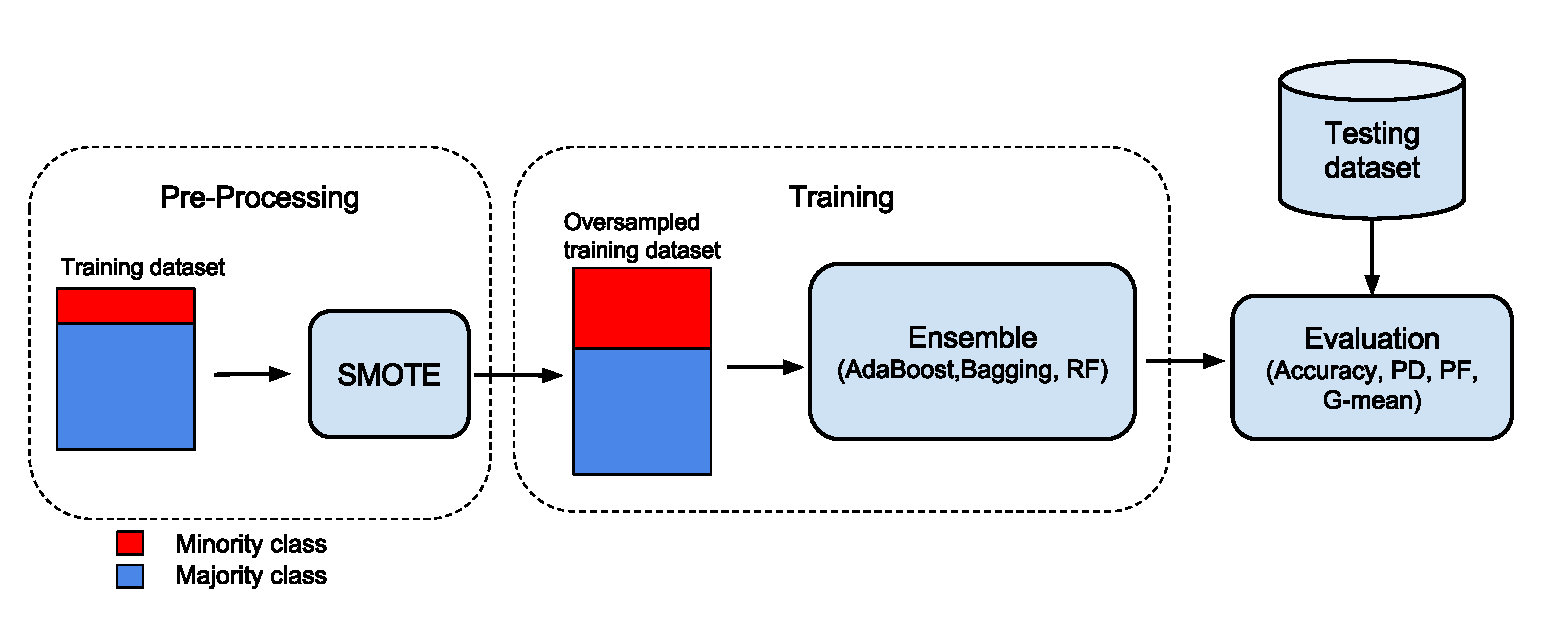
\includegraphics[scale=0.45]{Framework.eps}
\caption{Hybrid SMOTE-Ensemble approach for bug prediction}
\end{center}
\label{fig:confusion}
\end{figure}


\section{Datasets Description}
\label{data}


To facilitate the replication and verification of our experiments, four public benchmark datasets from REPOSITORY of NASA were used [1 ,].These datasets were collected from real software projects by NASA which were developed in C/C++ for spacecraft instrumentation (CM1 dataset), storage management of ground data (KC1 dataset), scientific data processing (JM1 dataset), and satellite flight control (PC3 dataset). The buggy rates of the datasets have a minimum value of 9.83\% and a maximum value of 19.35\%. The number of instances of the datasets is different. Each instance in the first three datasets CM1, KC1, and JM1 datasets includes total 22 attributes, of which five are different lines of code measure, three are McCabe metrics, four are base Halstead measures, eight are derived Halstead measures, one is a branch-count, and one is a decision attribute. PC3 is the last dataset and it includes 38 attributes, of which one is a decision attribute. Table 1 shows the detailed information of each dataset.


\begin{table}
\caption{Datasets information}
\begin{centering}
\begin{tabular}{|c|c|>{\centering}p{3cm}|c|c|c|c|c|c|c|}
\hline 
Dataset & Lang. & Description & No. of att. & LOC & No. of Mod. & Non-def. & Def. & \% Non-def. & \% Def.\tabularnewline
\hline 
\hline 
CM1 & C & NASA spacecraft instrument & 22 & 20K & 498 & 449 & 49 & 90.16 & 9.83\tabularnewline
\hline 
KC1 & C++ & System implementing storage management for receiving and processing
ground data & 22 & 43K & 2109 & 1783 & 326 & 84.54 & 15.45\tabularnewline
\hline 
JM1 & C & Real-time predictive ground system: Uses simulations to generate predictions & 22 & 315K & 10885 & 8779 & 2106 & 80.65 & 19.35\tabularnewline
\hline 
PC3 & C & Flight software for earth orbiting satellite metadata & 38 & 40K & 1563 & 1403 & 160 & 89.7 & 10.23\tabularnewline
\hline 
\end{tabular}
\par\end{centering}

\end{table}




\section{Model evaluation}
\label{evaluation_criteria}
In order to evalute the performance of the software faults prediction model, we used the confusion matrix that shown in Figure \ref{fig:confusion}, which is a table that is often used to describe the classfication model results. 

\begin{figure}[h]
\label{fig:ss}
\begin{center}
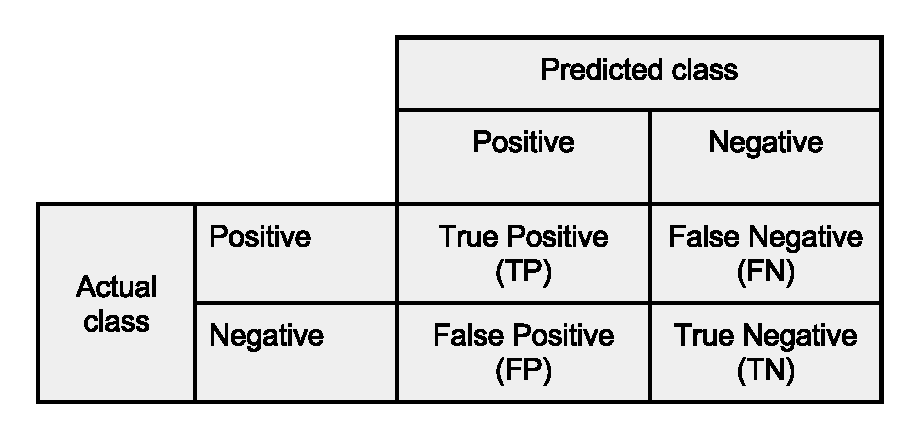
\includegraphics[scale=0.5]{confusion-matrix.eps}
\caption{Confusion matrix}
\end{center}
\label{fig:confusion}
\end{figure}

The bug detection effectiveness is evaluated using four measurements based on the previous confusion matrix; namely, Model Accuracy (Acc), Number of Predicted Defects (PD), Numebr of Incorectly Predicted cases with No Defects (PF), G-mean. Acc is the ratio of the correctly predicted faults to the total number of faults. PD is
the ratio of correctly predicted faults to the total number of faults. PF is the number of not fault-prone modules that are predicted incorrectly as defectes. In addtion, we used the G-mean to combine the PD and PF which is a good indicator of the relationship between the two measures. The PD, PF, G-mean are calculated in Equations \ref{accuracy}, \ref{PD}, \ref{PF}, and \ref{gmean}, respectively.

\begin{equation}
Accuracy=\frac{TP+TN}{TP + FN + FP + TN}
\label{accuracy}
\end{equation}

\begin{equation}
PD=\frac{TP}{TP+FN}
\label{PD}
\end{equation}

\begin{equation}
PF=\frac{FP}{FP+TN}
\label{PF}
\end{equation}

\begin{equation}
G-mean=\sqrt{PD \times (1-PF)}
\label{gmean}
\end{equation}

%%%%%%%%%%%%%%%%%%%%%%%%%%%%%%%%%%%%%%%%%%%%


%%%%%%%%%%%%%%%%%%%%%%%%%%%%%%%%%%%%%%%%%%%%

%==================================================================
\section{Experiments and Results}
\label{experiments}



 

%%%%%%%%%%%%%%%%%%%%%%%%%%%%%%
\begin{figure*}[http]
	\scalebox{0.75}{
		\begin{tabular}{p{5cm} p{4cm} p{5cm} }
			\centering
			
			%\subfigure[Appendicitis]{\label{fig:a}\includegraphics[scale=0.40]{appendicitis}}& &
			\subfigure[CM1]{\label{fig:a}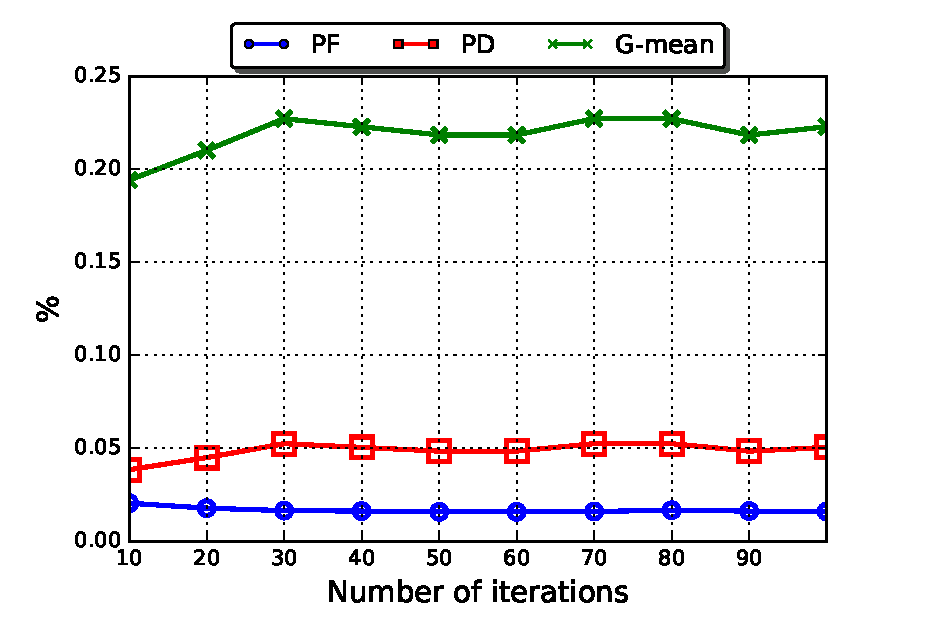
\includegraphics[scale=0.45]{RF-CM1}}& &
			\subfigure[JM1]{\label{fig:a}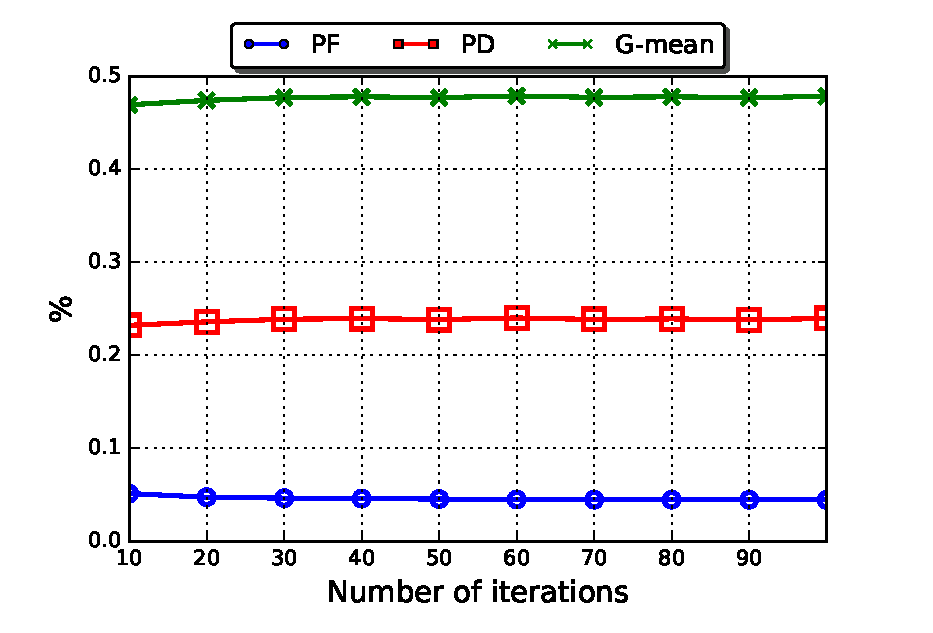
\includegraphics[scale=0.45]{RF-JM1}}

			\vspace{-1.5in}
			\\
			\subfigure[KC1]{\label{fig:a}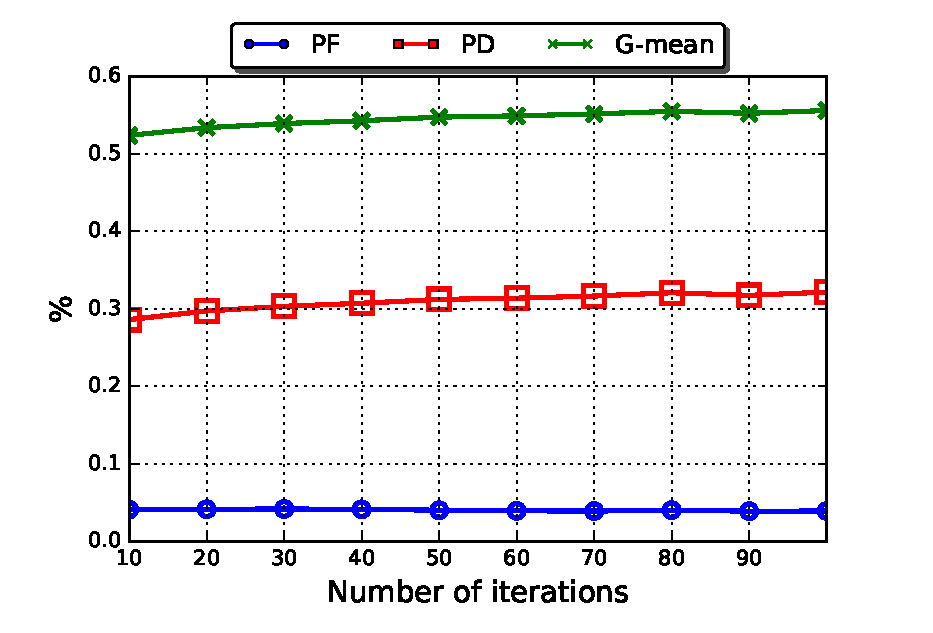
\includegraphics[scale=0.45]{RF-KC1}}& &
			\subfigure[PC3]{\label{fig:a}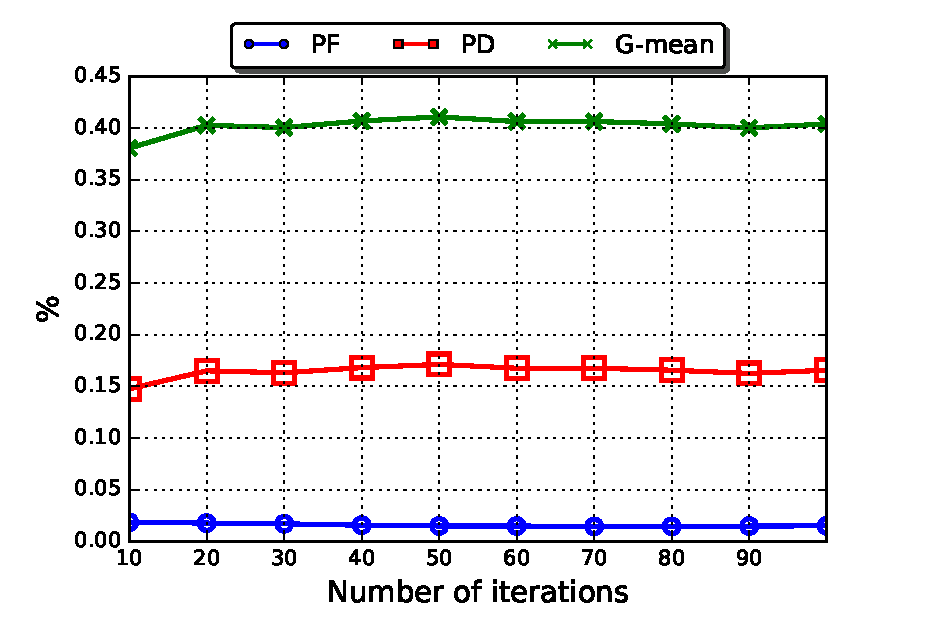
\includegraphics[scale=0.45]{RF-PC3}}

			\vspace{-1.5in}
			\\
%				
		\end{tabular}
	}
	\caption{Evaluation results of RF by changing number of iterations.}
	\label{fig:bestneurons}
	\vspace{-0.0in}
\end{figure*}
%%%%%%%%%%%%%%%%%%%%%%%%%%%%%%%%%%%%%%%%%%%

\begin{figure*}[http]
	\scalebox{0.75}{
		\begin{tabular}{p{5cm} p{4cm} p{5cm} }
			\centering
			
			%\subfigure[Appendicitis]{\label{fig:a}\includegraphics[scale=0.40]{appendicitis}}& &
			\subfigure[CM1]{\label{fig:a}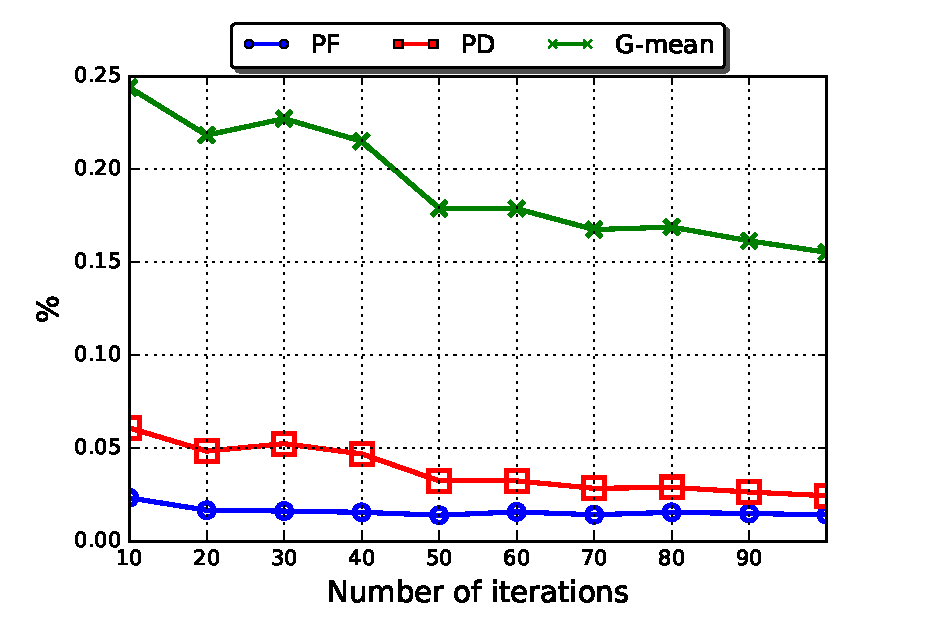
\includegraphics[scale=0.45]{Bagging-CM1}}& &
			\subfigure[JM1]{\label{fig:a}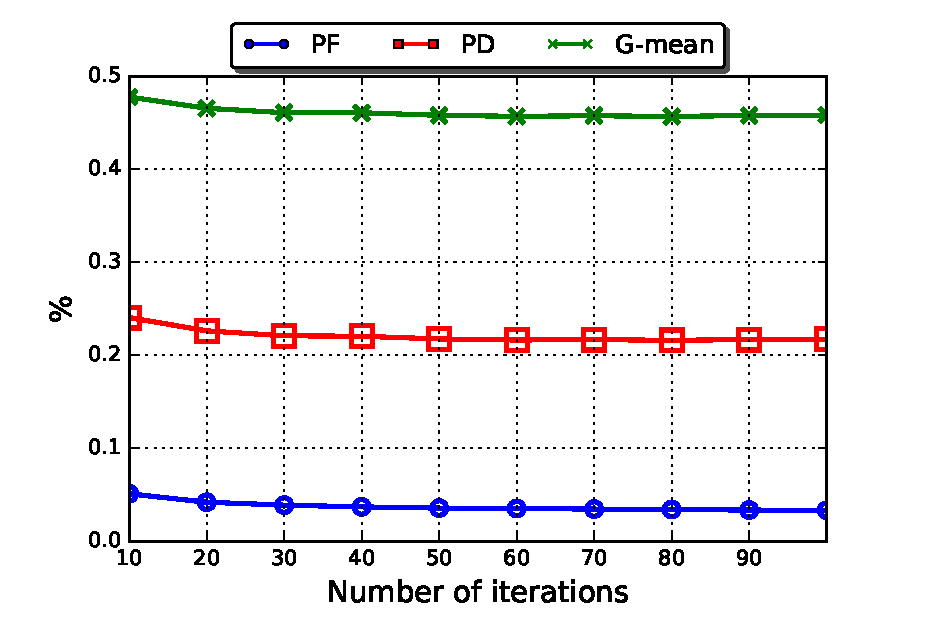
\includegraphics[scale=0.45]{Bagging-JM1}}

			\vspace{-1.5in}
			\\
			\subfigure[KC1]{\label{fig:a}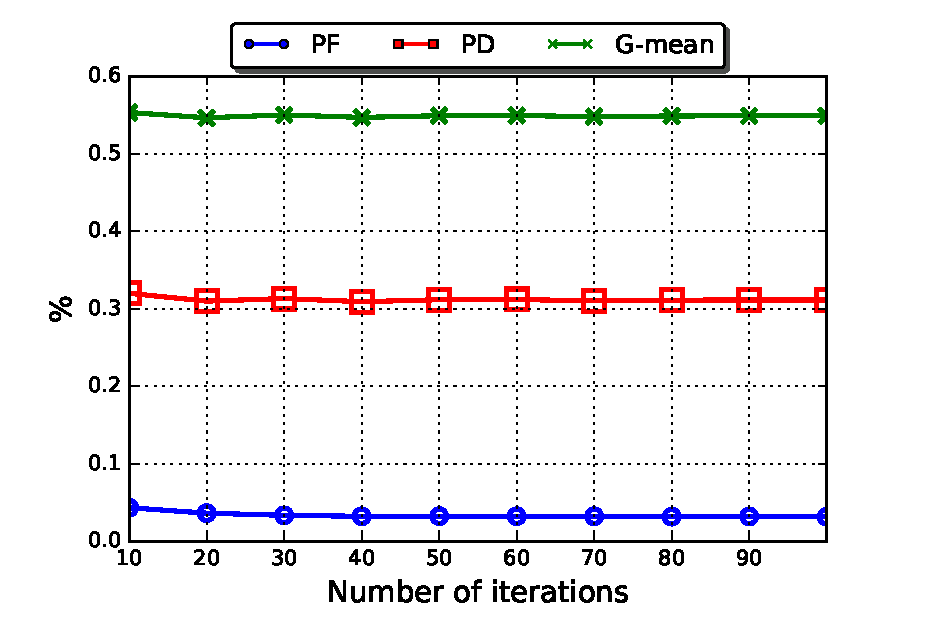
\includegraphics[scale=0.45]{Bagging-KC1}}& &
			\subfigure[PC3]{\label{fig:a}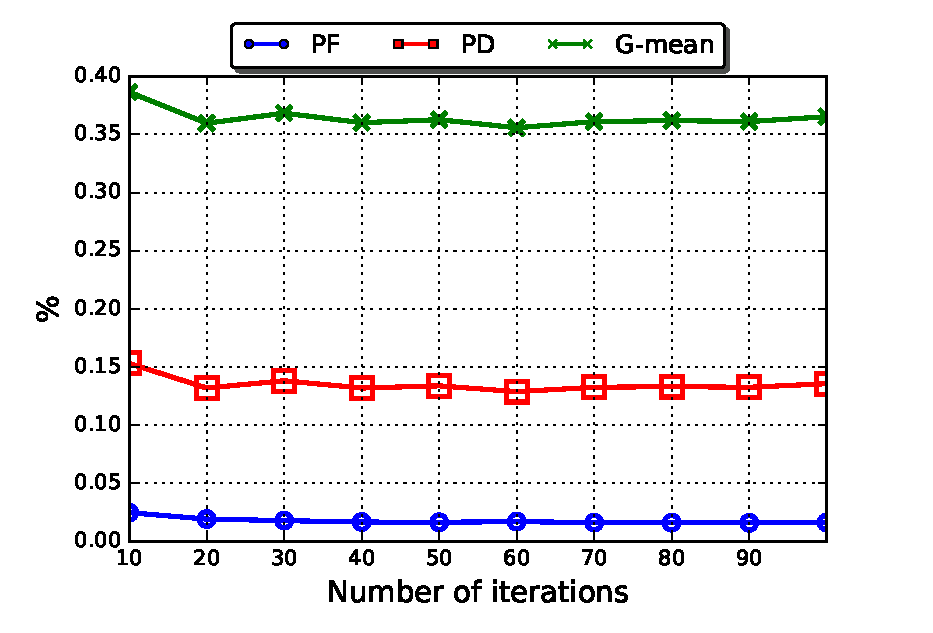
\includegraphics[scale=0.45]{Bagging-PC3}}

			\vspace{-1.5in}
			\\
%				
		\end{tabular}
	}
	\caption{Evaluation results of Bagging by changing number of iterations.}
	\label{fig:bestneurons}
	\vspace{-0.0in}
\end{figure*}
%%%%%%%%%%%%%%%%%%%%%%%%%%%%%%%%%%%%%%%%%%%

\begin{figure*}[http]
	\scalebox{0.75}{
		\begin{tabular}{p{5cm} p{4cm} p{5cm} }
			\centering
			
			%\subfigure[Appendicitis]{\label{fig:a}\includegraphics[scale=0.40]{appendicitis}}& &
			\subfigure[CM1]{\label{fig:a}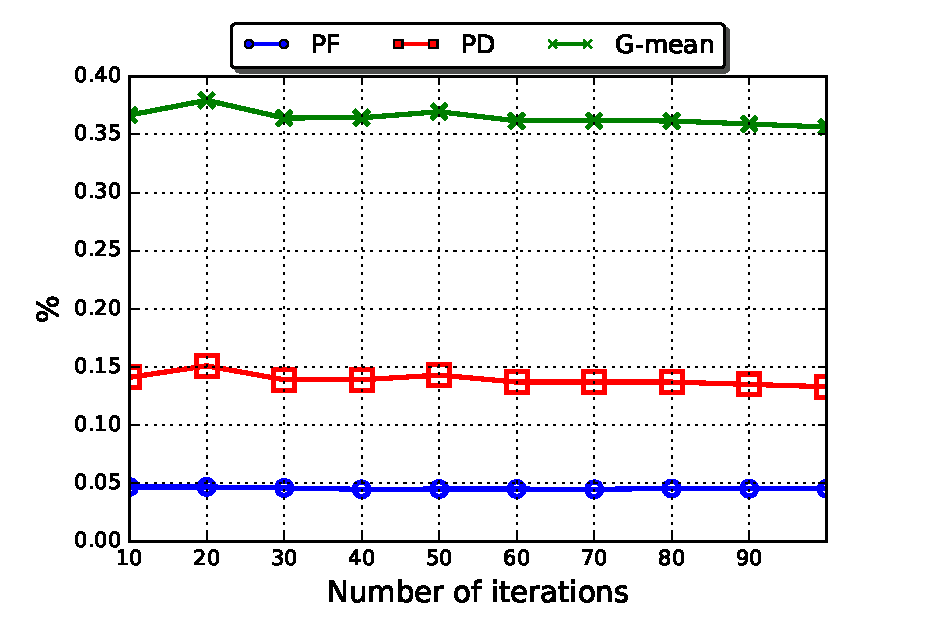
\includegraphics[scale=0.45]{AdaBoost-CM1}}& &
			\subfigure[JM1]{\label{fig:a}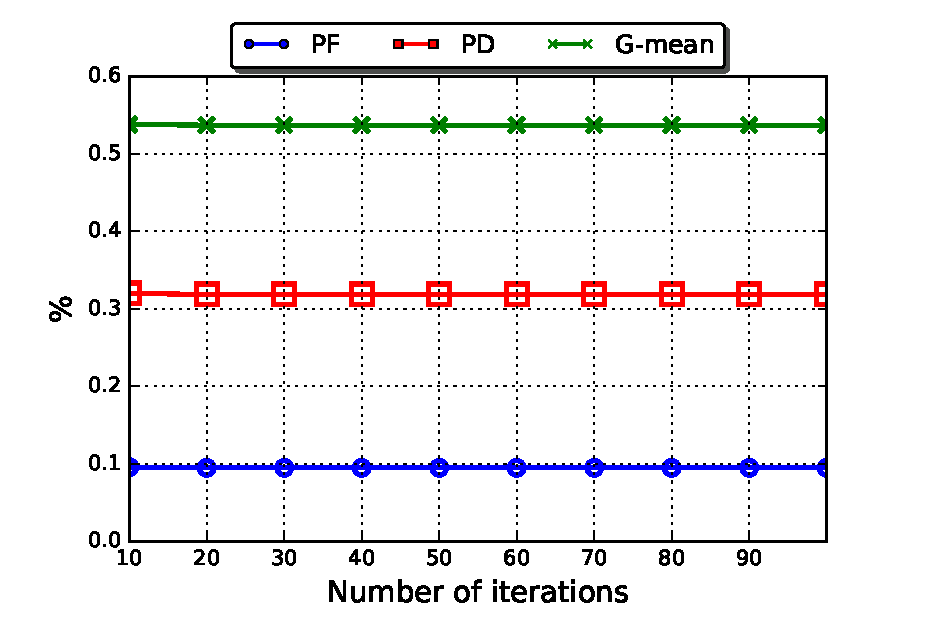
\includegraphics[scale=0.45]{AdaBoost-JM1}}

			\vspace{-1.5in}
			\\
			\subfigure[KC1]{\label{fig:a}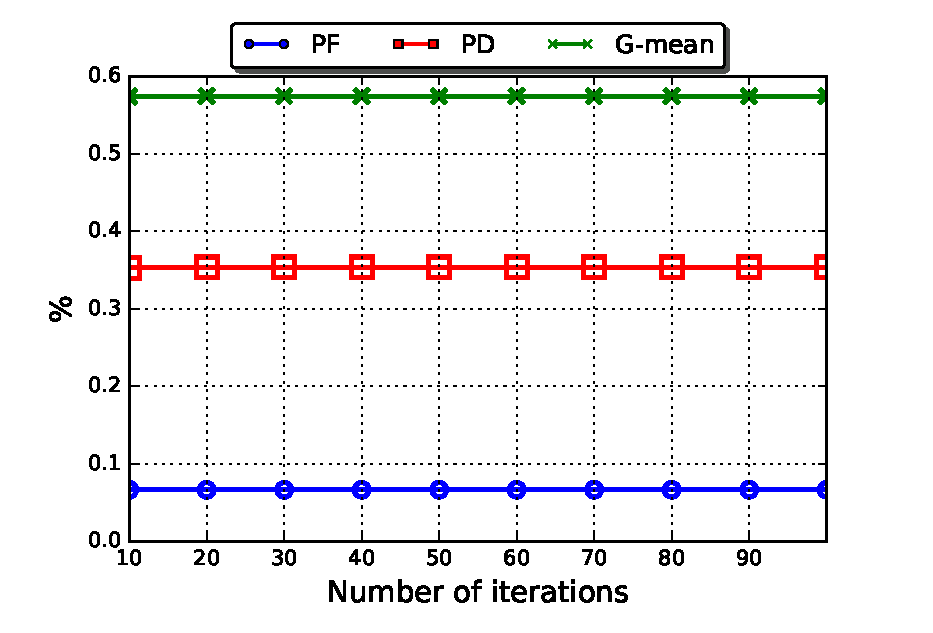
\includegraphics[scale=0.45]{AdaBoost-KC1}}& &
			\subfigure[PC3]{\label{fig:a}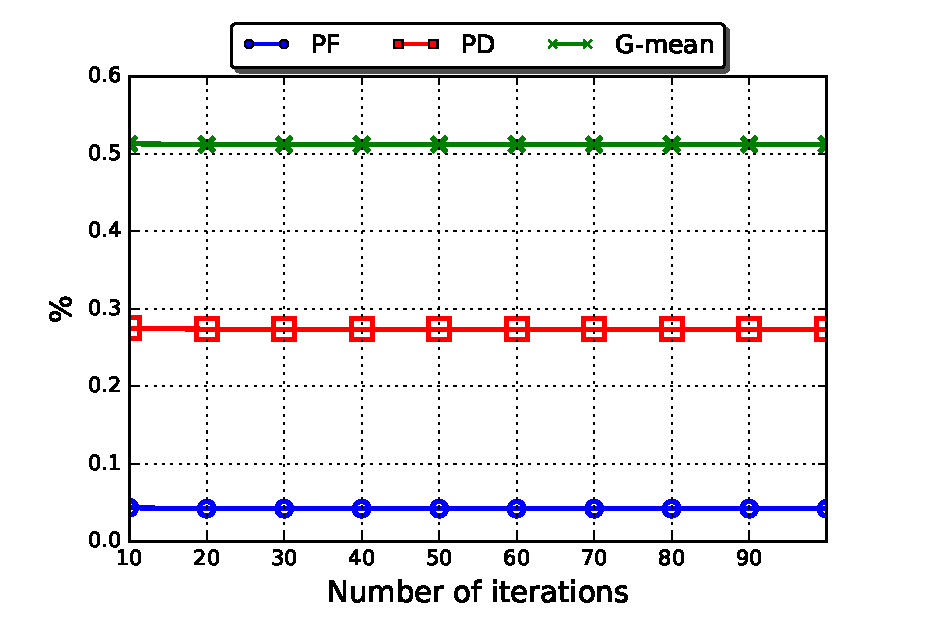
\includegraphics[scale=0.45]{AdaBoost-PC3}}

			\vspace{-1.5in}
			\\
%				
		\end{tabular}
	}
	\caption{Evaluation results of AdaBoost by changing number of iterations.}
	\label{fig:bestneurons}
	\vspace{-0.0in}
\end{figure*}

%%%%%%%%%%%%%%%%%%%%%%%%%%%%%%%%%%%%%%%%%%%

\begin{figure*}[http]
	\scalebox{0.75}{
		\begin{tabular}{p{5cm} p{4cm} p{5cm} }
			\centering
			
			%\subfigure[Appendicitis]{\label{fig:a}\includegraphics[scale=0.40]{appendicitis}}& &
			\subfigure[CM1]{\label{fig:a}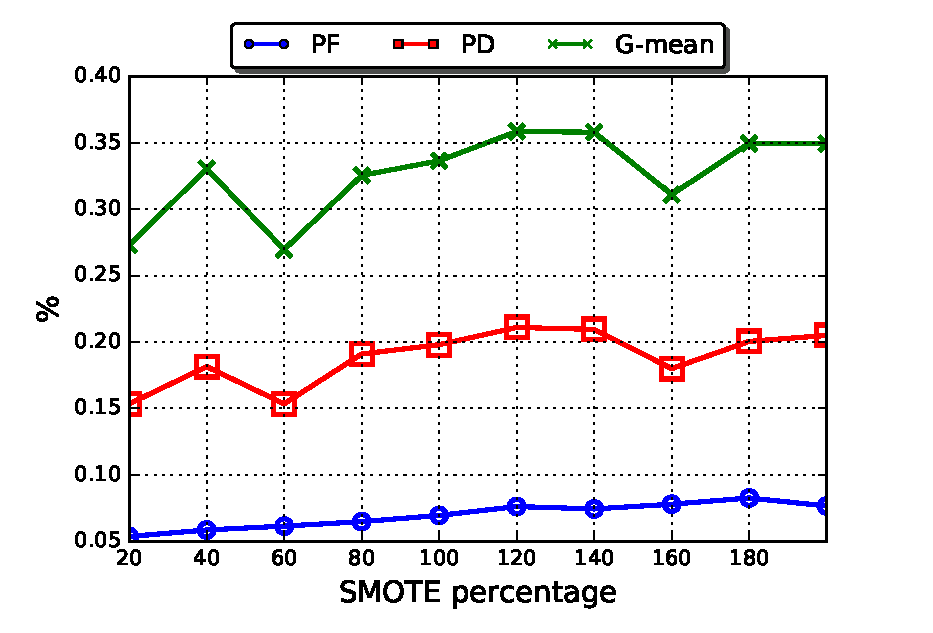
\includegraphics[scale=0.45]{SMOTE-AdaBoost-CM1}}& &
			\subfigure[JM1]{\label{fig:a}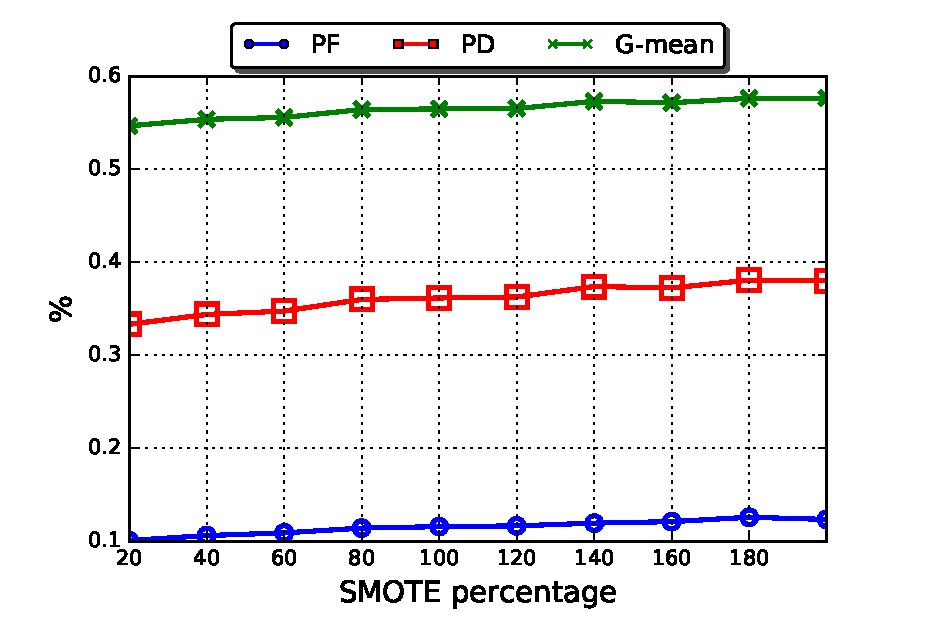
\includegraphics[scale=0.45]{SMOTE-AdaBoost-JM1}}

			\vspace{-1.5in}
			\\
			\subfigure[KC1]{\label{fig:a}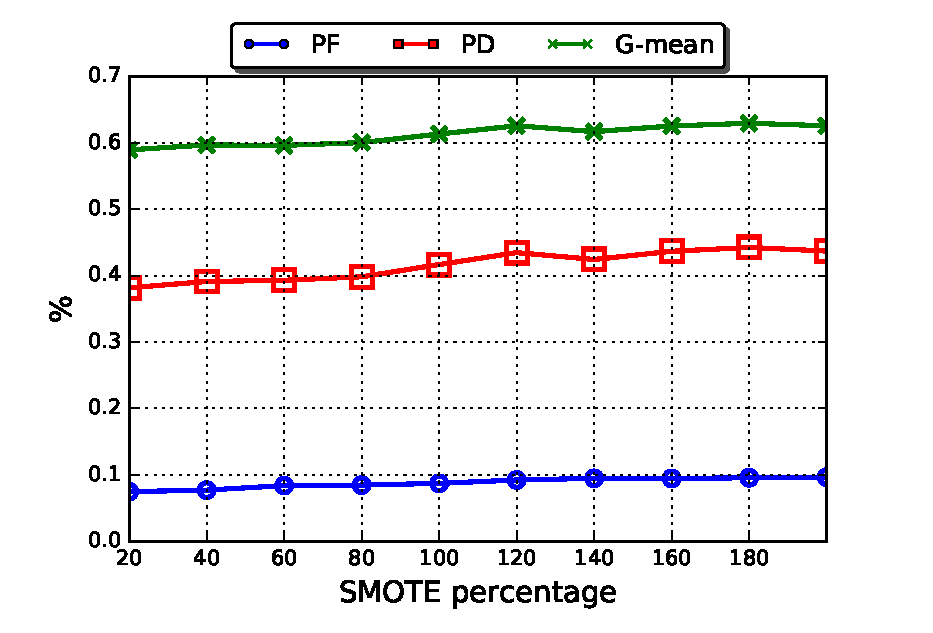
\includegraphics[scale=0.45]{SMOTE-AdaBoost-KC1}}& &
			\subfigure[PC3]{\label{fig:a}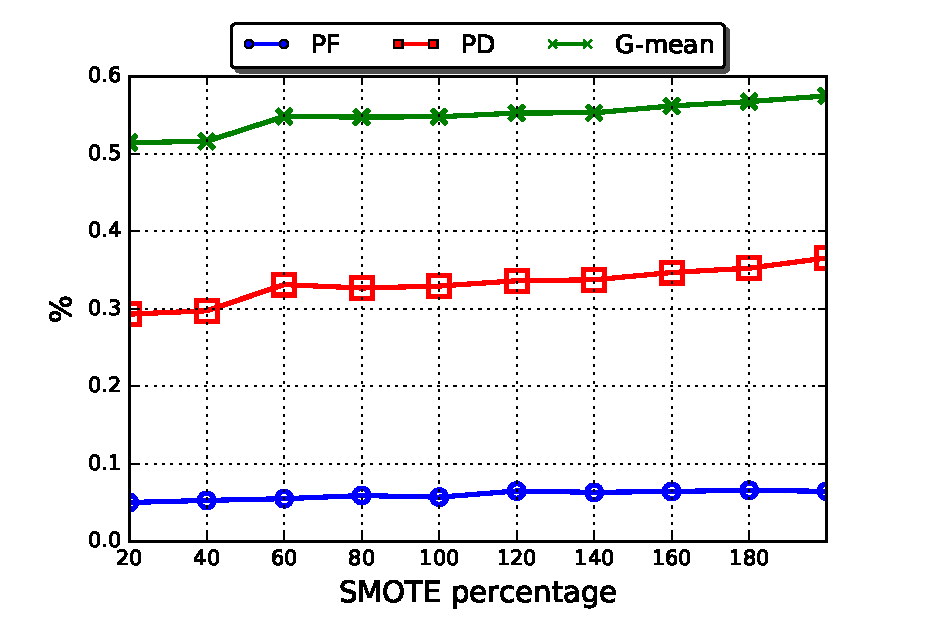
\includegraphics[scale=0.45]{SMOTE-AdaBoost-PC3}}

			\vspace{-1.5in}
			\\
%				
		\end{tabular}
	}
	\caption{Evaluation results of SMOTE+AdaBoost by changing number of iterations.}
	\label{fig:bestneurons}
	\vspace{-0.0in}
\end{figure*}


\begin{table}


\caption{Evaluation results for PC3 dataset}


\begin{centering}
\begin{tabular}{|c|c|c|c|c|c|}
\hline 
 & Accuracy & PF & PD & G-mean & AUC\tabularnewline
\hline 
\hline 
NB & 0.4826 & 0.5589 & 0.8469 & 0.6112 & 0.7668\tabularnewline
\hline 
J48 & 0.8814 & 0.0418 & 0.2081 & 0.4466 & 0.6304\tabularnewline
\hline 
MLP & 0.8820 & 0.0378 & 0.1788 & 0.4147 & 0.7812\tabularnewline
\hline 
RF & 0.9018 & 0.0149 & 0.1713 & 0.4107 & 0.8418\tabularnewline
\hline 
Bagging & 0.8912 & 0.0247 & 0.1531 & 0.3865 & 0.8195\tabularnewline
\hline 
AdaBoost & 0.8869 & 0.0433 & 0.2750 & 0.5129 & 0.8031\tabularnewline
\hline 
SMOTE+AdaBoost & 0.8772 & 0.0645 & 0.3656 & 0.5748 & 0.8106\tabularnewline
\hline 
\end{tabular}
\par\end{centering}
\end{table}


\begin{table}
\caption{Evaluation results for KC1 dataset}
\begin{centering}
\begin{tabular}{|c|c|c|c|c|c|}
\hline 
 & Accuracy & PF & PD & G-mean & AUC\tabularnewline
\hline 
\hline 
NB & 0.8246 & 0.0925 & 0.3715 & 0.5806 & 0.7909\tabularnewline
\hline 
J48 & 0.8404 & 0.0601 & 0.2964 & 0.5278 & 0.6963\tabularnewline
\hline 
MLP & 0.8565 & 0.0229 & 0.1963 & 0.4380 & 0.7852\tabularnewline
\hline 
RF & 0.8610 & 0.0402 & 0.3208 & 0.5548 & 0.8252\tabularnewline
\hline 
Bagging & 0.8582 & 0.0434 & 0.3200 & 0.5533 & 0.8123\tabularnewline
\hline 
AdaBoost & 0.8438 & 0.0665 & 0.3534 & 0.5743 & 0.7477\tabularnewline
\hline 
SMOTE+AdaBoost & 0.8329 & 0.0957 & 0.4424 & 0.6294 & 0.7700\tabularnewline
\hline 
\end{tabular}
\par\end{centering}
\end{table}


\begin{table}
\caption{Evaluation results for CM1 dataset}
\begin{centering}
\begin{tabular}{|c|c|c|c|c|c|}
\hline 
 & Accuracy & PF & PD & G-mean & AUC\tabularnewline
\hline 
\hline 
NB & 0.8484 & 0.0918 & 0.2985 & 0.5207 & 0.7382\tabularnewline
\hline 
J48 & 0.8805 & 0.0294 & 0.0550 & 0.2310 & 0.5591\tabularnewline
\hline 
MLP & 0.8825 & 0.0256 & 0.0400 & 0.1974 & 0.7586\tabularnewline
\hline 
RF & 0.8920 & 0.0165 & 0.0525 & 0.2272 & 0.7430\tabularnewline
\hline 
Bagging & 0.8865 & 0.0234 & 0.0610 & 0.2441 & 0.7290\tabularnewline
\hline 
AdaBoost & 0.8743 & 0.0468 & 0.1510 & 0.3794 & 0.6977\tabularnewline
\hline 
SMOTE+AdaBoost & 0.8536 & 0.0762 & 0.2110 & 0.3585 & 0.7100\tabularnewline
\hline 
\end{tabular}
\par\end{centering}
\end{table}

\begin{table}
\caption{Evaluation results for JM1 dataset}
\begin{centering}
\begin{tabular}{|c|c|c|c|c|c|}
\hline 
 & Accuracy & PF & PD & G-mean & AUC\tabularnewline
\hline 
\hline 
NB & 0.8042 & 0.0507 & 0.1993 & 0.4350 & 0.6901\tabularnewline
\hline 
J48 & 0.7973 & 0.0688 & 0.2394 & 0.4722 & 0.6677\tabularnewline
\hline 
MLP & 0.8100 & 0.0148 & 0.0799 & 0.2806 & 0.7050\tabularnewline
\hline 
RF & 0.8167 & 0.0450 & 0.2402 & 0.4789 & 0.7527\tabularnewline
\hline 
Bagging & 0.8118 & 0.0511 & 0.2406 & 0.4778 & 0.7280\tabularnewline
\hline 
AdaBoost & 0.7912 & 0.0958 & 0.3199 & 0.5378 & 0.6951\tabularnewline
\hline 
SMOTE+AdaBoost & 0.7787 & 0.1259 & 0.3808 & 0.5764 & 0.6986\tabularnewline
\hline 
\end{tabular}
\par\end{centering}
\end{table}



\section{Conclusions}
\label{conclusion}




%\subsection*{Acknowledgments.} Authors would like to thank the Jordanian mobile telecommunication operator Umniah for providing the required technical assistance and the data for this developed research work.




\bibliographystyle{splncs}
\bibliography{ref}
\end{document}
